\Problem
{باندهای عملیاتی در شبکه‌های تلفن‌همراه}
{
نسل دو شبکه تلفن همراه در باندهای 900 الی 1800 مگاهرتز است.
نسل سه این شبکه در بازه فرکانسی 2100 الی 900 مگاهرتز وجود دارد.
نسل چهار در بازه 1800 الی 2600 مگاهرتز است.
نسل پنجم شامل موج‌های باند بالا یعنی 6 گیگاهرتز است. همچنین باند متوسط 2 الی 5.4 گیگاهرتز را شامل می‌شود و باند پایین زیر 3 گیگاهرتز را شامل می‌شود.

موارد ذکرشده در بالا کلیتی از این فرکانس‌ها بودند. موردی دیگر تاثیرگذار باند و شرکت مورد نظر است. در جدول زیر اطلاعات کامل‌تری آورده شده است.

\begin{figure}[H]
    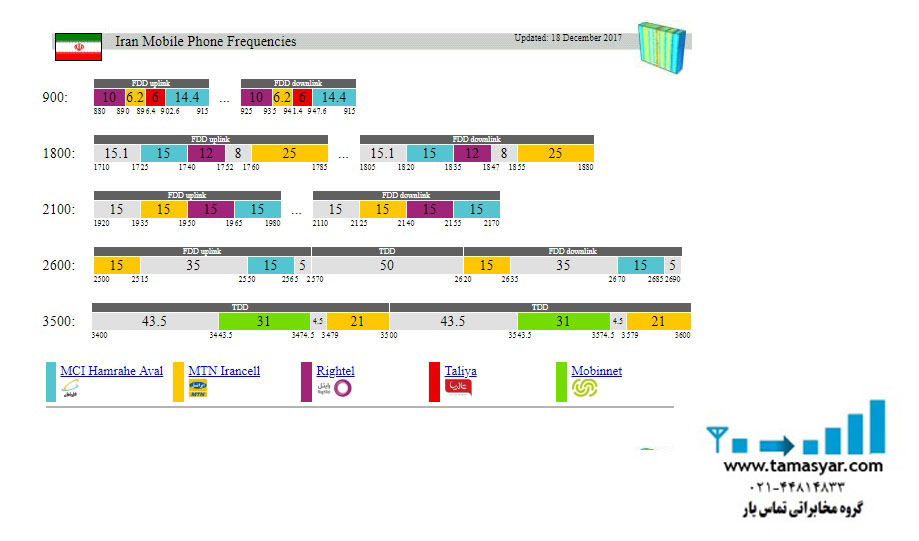
\includegraphics[width=15cm]{Images/Mobile-Frequencies-Iran.jpg}
    \centering
    \caption{\lr{Iran Mobile Frequencies}}
\end{figure}
}
